\documentclass[journal]{vgtc}                % final (journal style)
%\documentclass[review,journal]{vgtc}         % review (journal style)
%\documentclass[widereview]{vgtc}             % wide-spaced review
%\documentclass[preprint,journal]{vgtc}       % preprint (journal style)

%% Uncomment one of the lines above depending on where your paper is
%% in the conference process. ``review'' and ``widereview'' are for review
%% submission, ``preprint'' is for pre-publication, and the final version
%% doesn't use a specific qualifier.

%% Please use one of the ``review'' options in combination with the
%% assigned online id (see below) ONLY if your paper uses a double blind
%% review process. Some conferences, like IEEE Vis and InfoVis, have NOT
%% in the past.

%% Please note that the use of figures other than the optional teaser is not permitted on the first page
%% of the journal version.  Figures should begin on the second page and be
%% in CMYK or Grey scale format, otherwise, colour shifting may occur
%% during the printing process.  Papers submitted with figures other than the optional teaser on the
%% first page will be refused. Also, the teaser figure should only have the
%% width of the abstract as the template enforces it.

%% These few lines make a distinction between latex and pdflatex calls and they
%% bring in essential packages for graphics and font handling.
%% Note that due to the \DeclareGraphicsExtensions{} call it is no longer necessary
%% to provide the the path and extension of a graphics file:
%% \includegraphics{} is completely sufficient.
%%
\ifpdf%                                % if we use pdflatex
  \pdfoutput=1\relax                   % create PDFs from pdfLaTeX
  \pdfcompresslevel=9                  % PDF Compression
  \pdfoptionpdfminorversion=7          % create PDF 1.7
  \ExecuteOptions{pdftex}
  \usepackage{graphicx}                % allow us to embed graphics files
  \DeclareGraphicsExtensions{.pdf,.png,.jpg,.jpeg} % for pdflatex we expect .pdf, .png, or .jpg files
\else%                                 % else we use pure latex
  \ExecuteOptions{dvips}
  \usepackage{graphicx}                % allow us to embed graphics files
  \DeclareGraphicsExtensions{.eps}     % for pure latex we expect eps files
\fi%

%% it is recomended to use ``\autoref{sec:bla}'' instead of ``Fig.~\ref{sec:bla}''
\graphicspath{{figures/}{pictures/}{images/}{./}} % where to search for the images

\usepackage{microtype}                 % use micro-typography (slightly more compact, better to read)
\PassOptionsToPackage{warn}{textcomp}  % to address font issues with \textrightarrow
\usepackage{textcomp}                  % use better special symbols
\usepackage{mathptmx}                  % use matching math font
\usepackage{times}                     % we use Times as the main font
\renewcommand*\ttdefault{txtt}         % a nicer typewriter font
\usepackage{cite}                      % needed to automatically sort the references
\usepackage{tabu}                      % only used for the table example
\usepackage{booktabs}                  % only used for the table example
%% We encourage the use of mathptmx for consistent usage of times font
%% throughout the proceedings. However, if you encounter conflicts
%% with other math-related packages, you may want to disable it.

%% In preprint mode you may define your own headline.
%\preprinttext{To appear in IEEE Transactions on Visualization and Computer Graphics.}

%% If you are submitting a paper to a conference for review with a double
%% blind reviewing process, please replace the value ``0'' below with your
%% OnlineID. Otherwise, you may safely leave it at ``0''.
\onlineid{0}

%% declare the category of your paper, only shown in review mode
\vgtccategory{Research}
%% please declare the paper type of your paper to help reviewers, only shown in review mode
%% choices:
%% * algorithm/technique
%% * application/design study
%% * evaluation
%% * system
%% * theory/model
\vgtcpapertype{please specify}

%% Paper title.
\title{Improvements for PROACT}

%% This is how authors are specified in the journal style

%% indicate IEEE Member or Student Member in form indicated below
\author{Arthur Shing, Makiah Merritt, and Emmitt Johnson}
\authorfooter{
%% insert punctuation at end of each item
        \item
        Emmitt Johnson. E-mail: johnemmi@oregonstate.edu.
        \item
        Makiah Merritt. E-mail: merrittm@oregonstate.edu.
        \item
        Arthur Shing. E-mail: shinga@oregonstate.edu.
}

%other entries to be set up for journal
\shortauthortitle{Biv \MakeLowercase{\textit{et al.}}: Improvements for PROACTt}
%\shortauthortitle{Firstauthor \MakeLowercase{\textit{et al.}}: Paper Title}

%% Abstract section.
\abstract{
        PROACT (PROgnosis Assessment for Conservative Treatment) is a tool that helps patients figure out the prostate cancer health risks.
        We are aiming to come up with a way to visualize the adverse effects that patients may come across through various treatments.
        We had trouble finding data, so we ended up doing a simple visualization of treatment options as well as side effects. %
} % end of abstract

%% Keywords that describe your work. Will show as 'Index Terms' in journal
%% please capitalize first letter and insert punctuation after last keyword
\keywords{PROACT; Cancer; Visualization}

%% ACM Computing Classification System (CCS).
%% See <http://www.acm.org/class/1998/> for details.
%% The ``\CCScat'' command takes four arguments.

\CCScatlist{ % not used in journal version
 \CCScat{K.6.1}{Management of Computing and Information Systems}%
{Project and People Management}{Life Cycle};
 \CCScat{K.7.m}{The Computing Profession}{Miscellaneous}{Ethics}
}

%% Uncomment below to include a teaser figure.
\teaser{
  \centering
  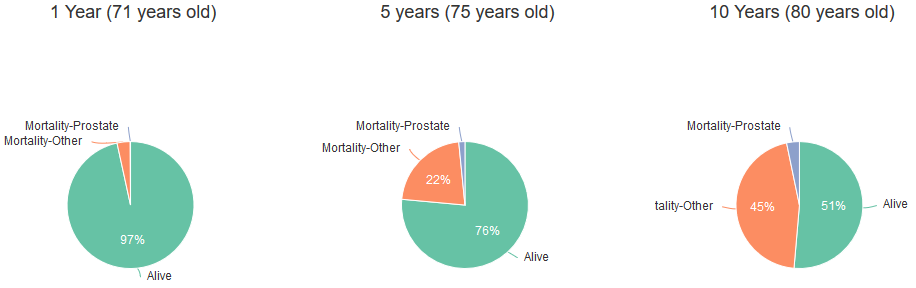
\includegraphics[width=\linewidth]{teaser}
  \caption{This teaser comes from the PROACT demo \cite{PROACTDemo:2016} and is showing the likelihood of dieing due to prostate cancer for a male of 70 years old in 1, 5, and 10 years.}
	\label{fig:teaser}
}

%% Uncomment below to disable the manuscript note
%\renewcommand{\manuscriptnotetxt}{}

%% Copyright space is enabled by default as required by guidelines.
%% It is disabled by the 'review' option or via the following command:
% \nocopyrightspace

\vgtcinsertpkg

%%%%%%%%%%%%%%%%%%%%%%%%%%%%%%%%%%%%%%%%%%%%%%%%%%%%%%%%%%%%%%%%
%%%%%%%%%%%%%%%%%%%%%% START OF THE PAPER %%%%%%%%%%%%%%%%%%%%%%
%%%%%%%%%%%%%%%%%%%%%%%%%%%%%%%%%%%%%%%%%%%%%%%%%%%%%%%%%%%%%%%%%

\begin{document}

%% The ``\maketitle'' command must be the first command after the
%% ``\begin{document}'' command. It prepares and prints the title block.

%% the only exception to this rule is the \firstsection command
\firstsection{Introduction}

\maketitle

%% \section{Introduction} %for journal use above \firstsection{..} instead
        This paper aims to make improvements on the PROACT paper.
        We first need to figure out where we can get the data for the visualizations.
        The information that needs to be gathered is data on side effects, recovery time, and quality of life.
        These are important things for people who are trying to figure out what treatments are best for them.
        After gathering this information we need to figure out the best way to display this back to the user. I
        t is important that we keep this visualization simple yet useful.
        The original paper made a big deal out of that, and we are hoping we can continue the great work they did.


\section{Related Work}
        \subsection{PROACT}
                PROACT (PROgnosis Assessment for Conservative Treatment) is a tool created and tested by Anzu Hakone, Lane Harrison, Alvitta Ottley, Nathan Winters, Caitlin Gutheil, Paul K. J. Han, Remco Chang to communicate risk information to individuals suffering from prostate cancer.
                ``PROACT utilizes two published clinical prediction models to communicate the patients’ personalized risk estimates and compare treatment options'' \cite[p.~1]{PROACT:2016}.
                With a primary goal of transmitting information across to emotionally charged individuals, the tool's design is backed by user studies of prostate cancer survivors and urologists from the Maine Medical Center.
                Through their study, they found an appropriate design required a easy to read bits of information that could likewise be easily comprehended with little effort.
                Specifically, listed in their \textit{findings} section, the team found a \textbf{temporal visualization} with \textbf{narrative sequence} worked best to communicate with varying \textbf{emotional state}s \cite[p.~8]{PROACT:2016}.
                This led the initial designs to use simple visualizations, such as pie and bar charts, minimal labeling, and present the data in a positive lens; noting ``adding interactions to either simple or complex visualizations had an adverse effect'' \cite[p.~2]{PROACT:2016}.

        \subsection{Health Care Visualizations}
                There have been many works that visualize medical data.
                Some of the examples listed in the PROACT paper include: "LifeLines [44], EventFlow [38], DecisionFlow [20], Outflow [52] and the system by Zhang et al. based on the five W’s [53]" \cite[p.~2]{PROACT:2016}.
                All of these works are important and bring something different to the table.
                LifeLines provides survival analysis which is mainly "developed to measure lifespans of individuals"\cite{LifeLines:2014}.
                This can be extremely beneficial to health care workers and scientists alike as it can provide the expected lifespan which gives the power to see if something is changing lifespans in a drastic way.
                The other papers and tools mentioned all have they own special area in which they help the community, and the PROACT team wanted to be apart of this as well.
                This is why they narrowed down their focus to prostate cancer as well as focusing on simple and effective feedback to their users.

\section{Implementation}
        Unfortunately, when searching for cancer data our team was only able to find resources concerning treatment options and a database outlining molecular trends of tumors.
        Coming across an accessible database was of particular interest as we would be able to provide accurate visualizations; however, the ones found were of no use for our scope.
        As such our ``implementation'' is not scientifically sound and will serve as a spring board for ideas.
        Noting the PROACT study found users didn't prefer interactive systems we desire to keep interactivity optional throughout the proposed solutions.
        We do feel, however, that interactive information is crucial to developing a better personal understanding of the presented information; and within a medical sense, the options one is able to pursue.

        \subsection{Additional or Alternative Treatments}
                As stated in many sources, including PROACT, there are many treatment paths for prostate cancer.
                The National Cancer Institute's (NCI) PDQ cancer information summary about prostate cancer states seven standard treatment options: active surveillance, surgery, radiation and radiopharmaceutical therapy, hormone therapy, chemotherapy, biologic therapy, and bisphosphate therapy \cite{PDQProstateCancer:2016}.
                Additionally, they list three new treatment options: cryosurgery, high-intensity-focused ultrasound therapy, and proton beam radiation therapy \cite{PDQProstateCancer:2016}.
                Of these PROACT currently observes conservative management (akin to active surveillance) and surgery.
                PROACTs lack of featuring additional treatments was cited as a possible improvement upon the current tool.
                By adding in other paths a patient might take, PROACT can better help doctors in providing all options with risk analysis.

                To facilitate additional paths, we would revise PROACT's \textit{Treatment Options} page to include statistics for these various measures.
                On the revised page users would be presented with an initial visualization comparing active and passive paths across the 1, 5, and 10 year spans currently depicted.
                Below this chart we propose adding toggle buttons allowing the user to create their own side by side survival/mortality rate comparisons.
                In addition to providing interactive comparisons, we propose the addition of \textit{Treatment Pathways}.
                With these an individual would be able to walk through the expected cycle of a selected treatment.
                During this walk, we would present information such as financing the treatment, possible side effects of the treatment, and resources for the treatment - including peer support groups and local organizations assisting in basic needs.
                An example of what this page might look like is shown in Figure \ref{fig:path}. As seen in the figure, colors could be added to codify larger or scientific terms.
                \begin{figure}[!ht]
                    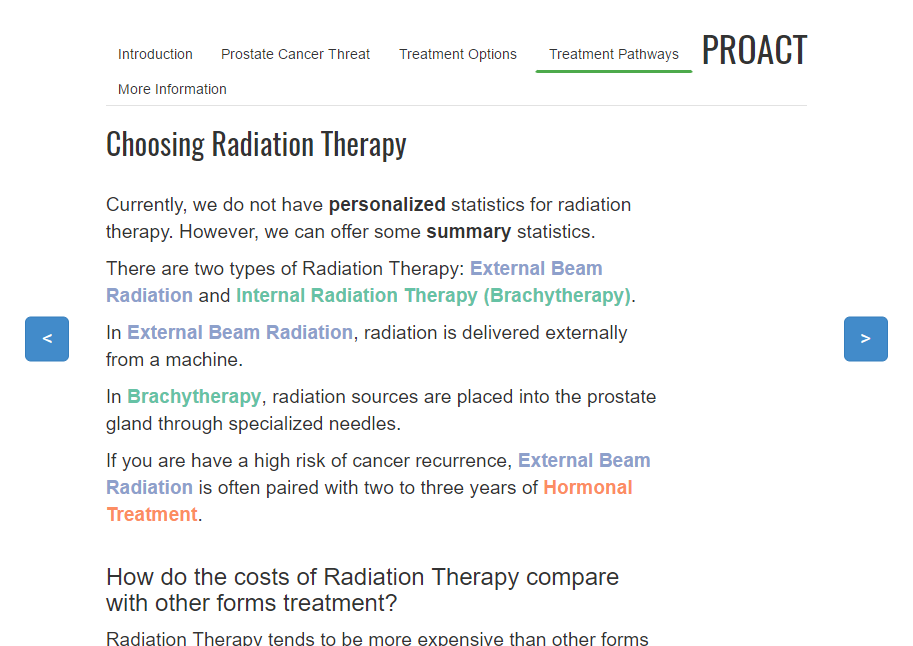
\includegraphics[width=\columnwidth]{pathway.png}
                    \caption{A prototype of the Treatment Pathways page.}
                    \label{fig:path}
                \end{figure}


        \subsection{Side Effects}
                Our vision for giving users visualizations of side effects associated with a prostate cancer would come in two forms.
                The addition would come in the form of an additional page titled ``Exploring Side Effects,'' appearing after PROACT's \textit{Treatment Options} page.
                Here the default view would be a visualization of the most prevalent side effects common across multiple treatment paths, i.e. erectile dysfunction or loss of bone mass.
                Then much like the proposed update to the \textit{Treatment Options} page, we would display buttons so users can explore the side effects of specific treatment paths.

                The following sections outline side effects we found for the surgical, hormonal therapy, and radiation therapy treatment options.
                Following side effects of individual treatment options, we have created a list of side effects common amongst multiple treatment options.
                The latter list would be served to users on our ``Exploring Side Effects'' page. We were able to implement a prototype of this page, shown in figure \ref{fig:side}.
                As seen below, indicative colors could be added to the frequency of side effects to denote the probability.
                \begin{figure}[!ht]
                    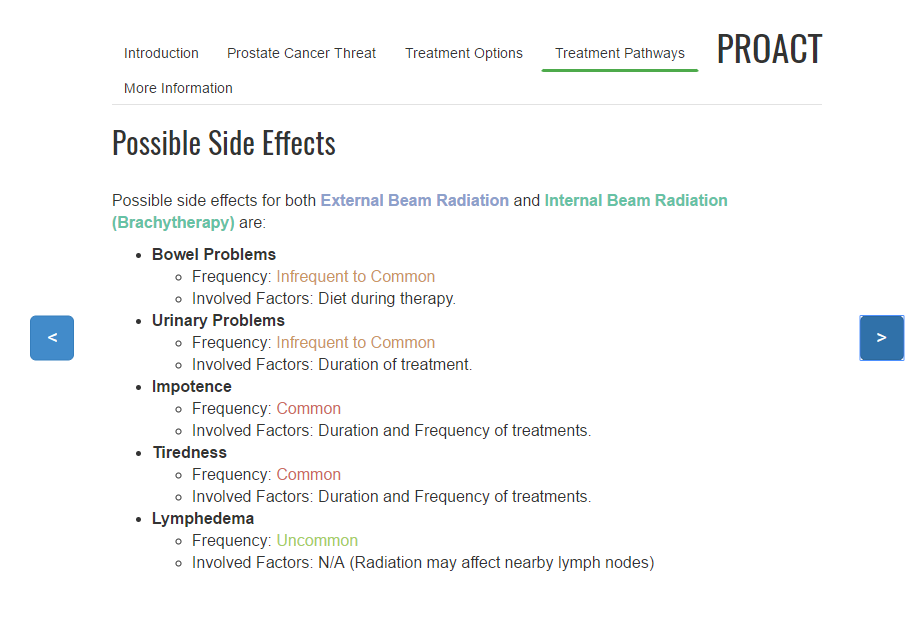
\includegraphics[width=\columnwidth]{sideeffects.png}
                    \caption{A prototype of the side effects page.}
                    \label{fig:side}
                \end{figure}

                \subsubsection{Surgery}
                        Surgeries for prostate cancer include \textit{radical prostatectomy} (with sub-types of \textit{retropubic prostatectomy} and \textit{retropubic prostatectomy}), \textit{pelvic lymphadenectomy}, and \textit{transurethral resection of the prostate (TURP)} \cite{PDQProstateCancer:2016}.
                        The following are some possible side effects: \\

                        \textbf{Pain}
                        \\ \textit{Frequency:} Common.
                        \\ \textit{Additional Factors:} Location, amount of tissue removed, incision size.
                        \newline

                        \textbf{Fatigue}
                        \\ \textit{Frequency:} Common.
                        \\ \textit{Additional Factors:} Loss of appetite, stress, anesthesia.
                        \newline

                        \textbf{Numbness}
                        \\ \textit{Frequency:} Common.
                        \\ \textit{Additional Factors:} N/A.
                        \\ Numbness is caused by skin nerves being cut during surgery.
                        \newline

                        \textbf{Swelling/Bruising}
                        \\ \textit{Frequency:} Common.
                        \\ \textit{Additional Factors:} N/A.
                        \newline



                \subsubsection{Hormonal Therapy}
                        The following is a list a list of possible side effects that individuals undergoing, or having undergone, hormonal therapy (a.k.a. androgen deprivation therapy) might face;  based upon the research presented in \textit{Adverse Events Associated with Hormonal Therapy for Prostate Cancer}\cite{AdverseEvents:2005}.
                        \newline

                        \textbf{Neurologic and Psychiatric Effects}
                        \\ \textit{Frequency:} Minor manifestation.
                        \\ \textit{Additional Factors:} N/A.
                        \\ As a hormonal therapy is manipulating an individuals chemical balances, neurologic and psychiatric effects are manifested in impairments to memory, concentration, verbal, and other cognitive skills and will affect emotions to some degree \cite{AdverseEvents:2005}.
                        \newline

                        \textbf{Hot Flushes}
                        \\ \textit{Frequency:} Common.
                        \\ \textit{Additional Factors:} N/A.
                        \\ Hot flashes are commonly reported and are risky to treat \cite{AdverseEvents:2005}.
                        \newline

                        \textbf{Gastrointestinal Side Effects}
                        \\ \textit{Frequency:} Common.
                        \\ \textit{Additional Factors:} Combination therapy, especially the use of luteinizing hormone-releasing hormone(LHRH).
                        \\ Similar to neurological and psychiatric effects, gastrointestinal effects are caused by the manipulation of an individuals natural chemical balances and are commonly ``abdominal pain, diarrhea and constipation, nausea/vomiting, and anorexia'' \cite{AdverseEvents:2005}.
                        \newline

                        \textbf{Musculoskeletal Side Effects}
                        \\ \textit{Frequency:} Minor manifestation, ``0.5\% - 1\% per year for older men'' \cite{AdverseEvents:2005}.
                        \\ \textit{Additional Factors:} Age and combination therapy.
                        \\ Typically seen as decreased muscle mass, increased fatigue, and decreased bone mineral density (BMD).
                        A chain effect, for older men, is an increased risk for osteoporosis and bone fractures. \cite{AdverseEvents:2005}
                        \newline

                        \textbf{Endocrine Side Effects}
                        \\ \textit{Frequency:} Infrequent to common.
                        \\ \textit{Additional Factors:} Type of hormonal therapy.
                        \\ With the manipulation of the bodies androgens, individuals are at a higher risk of developing \textit{gynecomastia}.
                        Gynecomastia will typically cease after stopping hormonal manipulation within the first year of appearance.
                        \newline

                        \textbf{Cardiovascular Side Effects}
                        \\ \textit{Frequency:} Common.
                        \\ \textit{Additional Factors:} N/A.
                        \\ With changes to the bodies chemical structure ones cholesterol level may also shift.
                        Therefore it isn't unlikely to see changes in weight or insulin levels. \cite{AdverseEvents:2005}
                        \newline

                        \textbf{Erectile Dysfunction}
                        \\ \textit{Frequency:} Very Common.
                        \\ \textit{Additional Factors:} N/A.
                        \\ A general loss of sexual desire and ability to generate/maintain an erection as well as changes to volume and rigidity of the erection is typically involved with the reduction of testosterone levels.
                        \newline

                        \textbf{Hematologic Adverse Effects}
                        \\ \textit{Frequency:} Common.
                        \\ \textit{Additional Factors:} Treatment type.
                        \\ Hormonal manipulation may cause hemoglobin levels to decrease resulting in a slightly increased chance of developing anemia. Any side effects however, can be mitigated if the hormonal treatment is stopped. \cite{AdverseEvents:2005}
                        \newline

                        \textbf{Biological Adverse Effects}
                        \\ \textit{Frequency:} Infrequent.
                        \\ \textit{Additional Factors:} Treatment type.
                        \\ With changes in testosterone levels, an individual might experience testosterone flares, ``body hair loss, dry eyes, and vertigo'' \cite{AdverseEvents:2005}.

                \subsubsection{Radiation Therapy}
                        Based upon the information provided by \textit{Radiation Therapy for Prostate Cancer}\cite{RadiationTherapy:2005} we gathered a list of possible side effects for individuals looking at radiation therapy.

                        The following have been outlined as possible side effects for both \textit{External Beam Radiation Therapy (EBRT)} and \textit{Internal Radiation Therapy (Brachytherapy)}.
                        \newline

                        \textbf{Bowel Problems}
                        \\ \textit{Frequency:} Infrequent to Common.
                        \\ \textit{Additional Factors:} Diet during therapy.
                        \\ Rectum irritation due to radiation can cause \textit{radiation proctitis}: ``diarrhea, (sometimes) blood in stool, and rectal leakage.'' \cite{RadiationTherapy:2005}
                        \newline

                        \textbf{Urinary Problems}
                        \\ \textit{Frequency:} Infrequent to Common.
                        \\ \textit{Additional Factors:} Duration of treatment.
                        \\ Bladder irritation (\textit{radiation cstitis}) or narrowing of the urethra (\textit{urethral stricture}) because of radiation can result in leakage and loss of bladder control, or inability to urinate (as in the case of a \textit{urethral stricture}). \cite{RadiationTherapy:2005}
                        \newline

                        \textbf{Erection Problems and Impotence}
                        \\ \textit{Frequency:} Common.
                        \\ \textit{Additional Factors:} Duration and frequency of treatments.
                        \\ Erectile Dysfunction (ED) may develop over the course of a patients undergoing yearly treatment. According to \textit{Radiation Therapy for Prostate Cancer} the frequency rates of ED rise to similar levels of patients who've had surgery for prostate cancer. \cite{RadiationTherapy:2005}
                        \newline

                        The following have been outlined as possible side effects for \textit{External Beam Radiation Therapy (EBRT)}.
                        \newline

                        \textbf{Tiredness}
                        \\ \textit{Frequency:} Common.
                        \\ \textit{Additional Factors:} Duration and frequency of treatments.
                        \\ As is the case with most radiation therapies, patients may feel fatigued due to the therapy destroying healthy cells in proximity to the targeted cancer cells; which the body must repair. \cite{RadiationTherapy:2005}
                        \newline

                        \textbf{Lymphedema}
                        \\ \textit{Frequency:} Uncommon.
                        \\ \textit{Additional Factors:} N/A.
                        \\ Radiation therapy may damage the lymph nodes around the prostate causing fluid to collect in the bodies lower regions. \cite{RadiationTherapy:2005}
                        \newline

                        The following have been outlined as possible side effects for \textit{Internal Radiation Therapy (Brachytherapy)}.
                        \newline

                        \textbf{Radiation}
                        \\ \textit{Frequency:} Uncommon.
                        \\ \textit{Additional Factors:} Type of brachytherapy.
                        \\ Due to the nature of brachytherapy individuals may give off trace amounts of radiation. \cite{RadiationTherapy:2005}
                        \newline

                \subsubsection{Common Side Effects}
                        \paragraph{Erectile Dysfunction (ED)}
                                Erectile dysfunction seems to be the most common side effect of prostate cancer treatments.
                                In the case of surgery, it is related to damaged nerves in the region as doctors perform their incisions. If present, signs of ED will typically arise quickly.
                                With hormonal therapy, it is typically caused by changes in testosterone levels and is potentially reversible.
                                Lastly, ED may develop with radiation therapy over time; with roughly the same frequency rates of surgery \cite{RadiationTherapy:2005}.

                        \paragraph{Bowel and Urinary Problems}
                                Bowel and urinary problems are the result of stress induced upon the rectum, bladder, or urethra.
                                The effects tend to be minor and are likely to go away in most cases.


        \subsection{Maintaining Utility}
                \subsubsection{Tool Tips}
                        The authors of PROACT did a great job of providing tool tips for possibly confusing articles of information.
                        As we researched additional treatment options and their side effects we found an increasing amount of technical and scientific information.
                        Because users are unlikely to know this information without looking it up and because a long scientific name could be daunting, we aim to extend the use of tool tips for any technical or scientific term.
                        With this users would hover over a term and a small dialog box would appear next to it.
                        In the dialog box we would present a high level definition of the term (for individuals with low literacy levels) as well as a link for more details - taking them to a resource appropriate for detailing the piece of medical information.
                        This would aid users who are viewing the PROACT tool without their doctor present.
                        An early prototype of the tooltip implementation can be seen on the Treatment Pathways page. As shown in Figure \ref{fig:tool}, upon hovering, a brief description for Internal Radiation Therapy is given.
                        \begin{figure}[!ht]
                            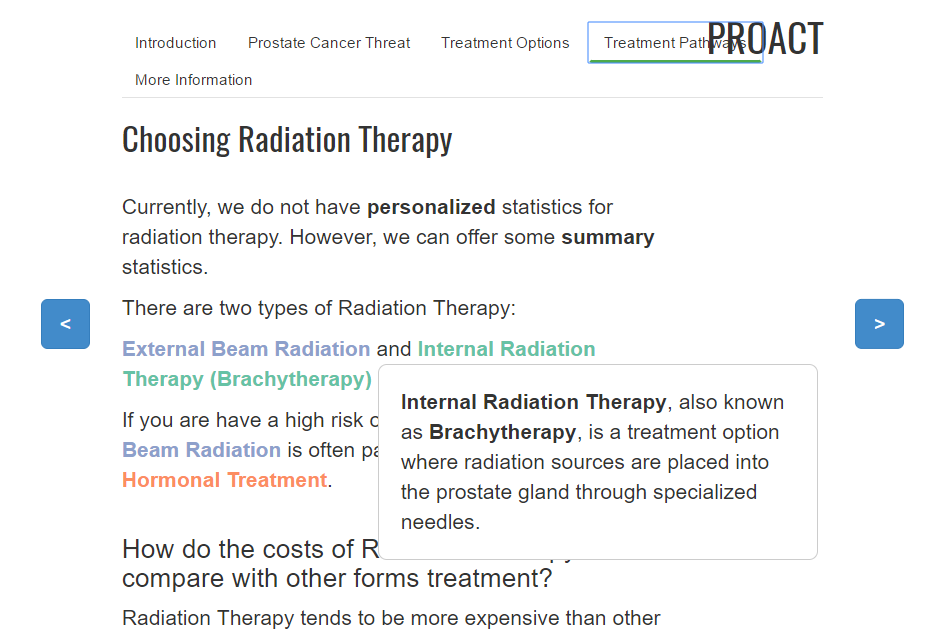
\includegraphics[width=\columnwidth]{tooltip.png}
                            \caption{An implementation of the tooltip feature.}
                            \label{fig:tool}
                        \end{figure}

                \subsubsection{Narrative Structure}
                        In addition, the PROACT authors emphasized the importance of creating a narrative flow that would allow the patient to feel at ease.
                        They found that creating a narrative structure that was conducive to a patient's psychological mindset was imperative for a good visualization tool.
                        To keep this flow, our additions to the Treatment Pathway page is an effort to aid the patient in following along in a calming manner.
                        We saw that the original, first-iteration implementation of PROACT by the researchers included some pages that disrupted this flow, and was removed in the second iteration.
                        Our addition of the treatment pathways page is an attempt to improve the flow by avoid blunt statistics and adding colors, as well as slightly more interaction through the tooltips.

                % \subsubsection{Minimization of Presented Data}


\section{Future Work}
        As the PROACT team has already performed the user studies necessary to outline what tool's functionality and narrative structure, future work primarily looks at the expansion of its current capabilities.

        \subsection{Data Collection}
                Although our work was able to identify and bring together the most common treatments and treatment side effects of prostate cancer, the sources used didn't provide frequency rates with which a usable visualization could be made.
                To delve further into this, research needs to be done to gather enough data to scientifically justify any numbers presented.
                The last portion of gathering data is factor analysis.
                As PROACT is a tool that tries to provide personalized predictions, it is necessary that newly added material conforms to this idea and that the data yields itself to providing predictions for patients.

        \subsection{PROACT Additions}
                We originally believed the code for PROACT to be open source, however, when looking at their GitHub repo \cite{PROACTDemo:2016}, only a demonstration and an unrelated page were publically accessible.
                To implement our suggestions one would of course need access to a dataset covering treatment survival rates and treatment side effect frequencies.
                As the PROACT team implements D3 in their current demo, creating a visualization with this dataset would be a trivial matter.

        \subsection{Visual Appeal}
                As the current PROACT tool is presented as a demonstration it is still very simple.
                To improve upon its appeal, an interface overhaul should be considered; while trying to maintain a similar sense of simplicity.
                Primary targets for overhaul would therefore be the improvement of navigation within the application, to make sure that users are aware of where they are at within the process at all times and how they can move on to the next section, or revisit a previous section.
                From usability studies we also know that a primary concern for male individuals is the use of colors.
                As such, the overhaul would also take a look at color palettes that could be implemented to allow the widest spectrum of users, without hassle.

\section{Conclusion}
        We have presented the work done by the PROACT team, and proposed a set of improvements to the visualization.
        These include the implementation of tooltips, an extensive section on other treatment options, a walkthrough of treatment options, and a walkthrough of possible side effects.
        While we were unable to effectively implement these due to a lack of resources and data, we were able to create an early prototype.
        This prototype included a brief side effects section and an example of what a treatment pathway page might look like.
%% if specified like this the section will be committed in review mode
\acknowledgments{
        The authors wish to thank Eugene Zhang for the unique opportunities provided in this class. We appreciate the work you are doing!
}

%\bibliographystyle{abbrv}
\bibliographystyle{abbrv-doi}
%\bibliographystyle{abbrv-doi-narrow}
%\bibliographystyle{abbrv-doi-hyperref}
%\bibliographystyle{abbrv-doi-hyperref-narrow}

\bibliography{references}
\end{document}
